\subsection{Self Training}
\label{sec:selftraining}

The method used for semi-supervised training is a modification of the
self-training approach described in \cite{vesely2013-semi}. In this
method, a multilingual DNN-HMM speech recognizer, trained on languages
other than the target language, is used to decode unlabelled audio in
the target language.  As shown in Fig.~\ref{fig:fig_hager}, decoding
results in a posterior probability $\pi(\phi_m^\ell|x_t^\ell)$ for
each frame $x_t^\ell$ of audio in the target language.

\begin{figure}
  \centerline{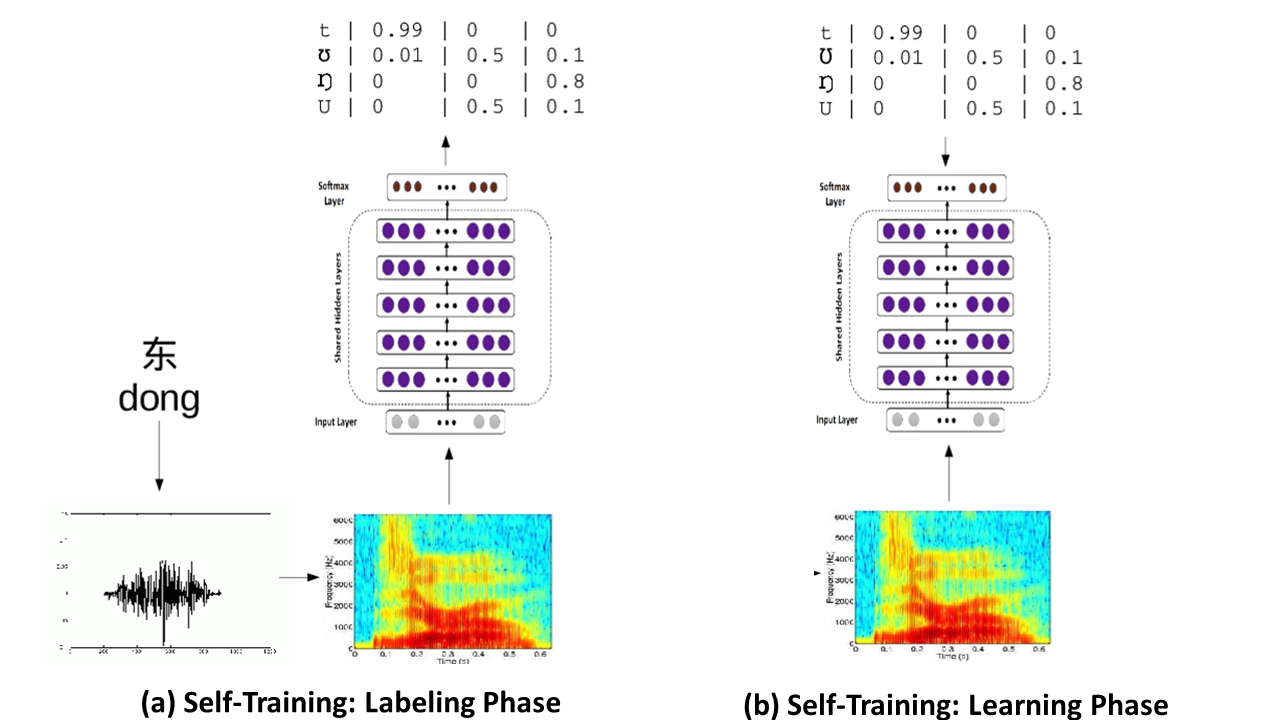
\includegraphics[width=5in]{../figs/fig_hager.png}}
  \caption{The self-training method of~\cite{vesely2013-semi} includes
    a labeling phase and a learning phase.  (a) Labeling phase: an ASR
    trained on other languages (here Cantonese) is used to compute
    posterior phone probabilities $\pi(\phi_t^\ell|x^\ell)$ in the
    test language (here Mandarin). (b) Learning phase: posterior phone
    probabilities are used as targets for DNN re-training.}
  \label{fig:fig_hager}
\end{figure}
%% comments: since the key difference in this figure between the
%% labeling phase and the learning phase is the direction of the upper
%% arrow, I suggest making the arrows more prominent. Also, the text
%% annotating the DNN is illegible, as is the text garnishing the axes
%% of the waveform and spectrograms.

In contrast to the approach in \cite{vesely2013-semi}, which used the
best path alignment as the target in frame cross-entropy training, we
achieved better performance using the posteriors as soft-targets
(Fig.~\ref{fig:fig_hager}). However, we did follow the recommendation in
\cite{vesely2013-semi} to scale the amount of transcribed data by 2 to 
create a good balance between transcribed and untranscribed data.
%% comment: the original text ("we empirically found it better") is
%% vague. My replacement ("we achieved better performance") is not much
%% improved. Would be good to provide more detail about how/why using
%% soft targets was better than using best path alignment.

The results on using this DNN are shown in Table \ref{tab:ptresult}. Although
semi-supervised training improves PER performance over multilingual DNN, it
still falls short of adaptation to probabilistic transcriptions (described in
Section \ref{sec:adaptation}). This is in spite of the untranscribed audio data
being several times larger than the probabilistic transcription data. Thus, we
show that mismatch transcripts can be more effective than ASR transcription for
training acoustic models.
%% Confused why results tables (tab:ptresult) are being mentioned here,
%% when the details of the experiment haven't been presented yet. It's
%% also generally dispreferred to reference a table several pages ahead
%% of its appearance in the manuscript.
%%
%% Also see comment in section s3_training_map regarding language
%% abbreviations with regard to tab:ptresult.
